\chapter{Application de la dérivation}
\thispagestyle{fancy}

%\vspace{-0.4cm}
\section{Étude des variations d'une fonction}

\begin{bthm}
	Soit une fonction $f$ définie et dérivable sur un intervalle I.
	\begin{itemProp}
		\item Si $f'(x)\leq 0$, alors $f$ est décroissante sur I.
		\item Si $f'(x)\geq 0$, alors $f$ est croissante sur I.
	\end{itemProp}
\end{bthm}

\subsection{Exemple d'une fonction du second degré}

\begin{bmethodet}{Étudier les variations d'une fonction polynôme du second degré}
\grasInMet{Enoncé :}
Soit la fonction f définie sur \R par $f(x)=2x^2-8x+1$.
\begin{enumMet}
	\item Calculer la fonction dérivée de $f$.
	\item Déterminer le signe de $f'$ en fonction de $x$.
	\item Dresser le tableau de variations de f.
\end{enumMet}
\ \\
%\newpage
\grasInMet{Réponse :}
\begin{enumMet}
\item Pour tout x réel, on a : $f'(x)=2\times 2x-8=4x-8$.
\item On commence par résoudre l'équation $f'(x)=0$.\\
Soit : $4x-8=0$\\
Donc $4x=8$  et $x= \dfrac{8}{4}=2$.\\
La fonction $f'$ est une fonction affine représentée par une droite dont le coefficient directeur 4 est positif.\\
Elle est donc d'abord négative (avant $x=2$) puis ensuite positive (après $x=2$).\\
%\newpage
\item On dresse alors le tableau de variations en appliquant le théorème :\\

\begin{center}
    \begin{tikzpicture}
        \tkzTabInit{$x$ / 0.8 , $f'(x)$ / 0.8, $f(x)$ / 1.4}{$-\infty$, $2$ ,$+\infty$}
        \tkzTabLine{, -,z , +,  }
        \tkzTabVar{+/  ,-/$-7$ ,  +/ }
    \end{tikzpicture}
	%\includegraphics[scale=1]{01-08-01.png}
\end{center}
\newpage
En effet : $f(2)=2\times 2^2-8\times 2+1=-7$.\\
La fonction f admet un minimum égal à $-7$ en $x=2$.\\
\end{enumMet}
\end{bmethodet}

\subsection{Exemple d'une fonction du troisième degré}

\begin{bmethodet}{Dresser le tableau de variations d'une fonction polynôme du 3e degré}
	Soit la fonction $f$ définie sur \R par $f(x)=x^3+\dfrac{9}{2} x^2-12x+5$.
	\begin{enumMet}
		\item Étudier les variations de $f$ et dresser le tableau de variation.
		\item Dans repère, représenter graphiquement la fonction f.
	\end{enumMet}
\ \\
\ \\
\begin{enumMet}
\item Pour tout $x$ réel, on a : $f'(x)=3x^2+9x-12$.\\
Commençons par résoudre l'équation $f'(x)=0$ :\\
Le discriminant du trinôme $3x^2+9x-12$ est égal à $\Delta = 92 - 4 \times 3 \times (–12) = 225$\\
L'équation possède deux solutions : $x_1= \dfrac{-9-\sqrt{225}}{2\times 3} = -4$ et $x_2= \dfrac{-9+\sqrt{225}}{2\times 3} = 1$\\
\\
On en déduit le tableau de variations de f :\\
\begin{center}
    \begin{tikzpicture}
        \tkzTabInit{$x$ / 0.8 , $f'(x)$ / 0.8, $f(x)$ / 2}{$-\infty$, $-4$,$1$ ,$+\infty$}
        \tkzTabLine{, +,z , -, z, +,  }
        \tkzTabVar{-/  ,+/$61$ ,  -/$-\dfrac{3}{2}$, +/ }
    \end{tikzpicture}
	%\includegraphics[scale=0.8]{01-08-02.png}
\end{center}
\item \ \\
\begin{center}
	\includegraphics[scale=0.8]{Img_01}
\end{center}
\end{enumMet}
\end{bmethodet}

\section{Extremum d'une fonction}

\begin{bthm}
	Soit une fonction $f$ définie et dérivable sur un intervalle ouvert I.
    Si la dérivée $f'$ de $f$ s'annule et change de signe en un réel $c$ de I alors $f$ admet un extremum en $x = c$.
\end{bthm}

\begin{bmethodet}{Rechercher un extremum}
\grasInMet{Enoncé :}\\
	La fonction f définie sur \R par $f(x)=5x^2-3x+4$ admet-elle un extremum sur \R ?\\
	\ \\
\grasInMet{Réponse :}\\
Pour tout x réel, on a : $f'(x)=10x-3$ \\
Et : $f'(x)=0$ pour $x=\dfrac{3}{10}$.\\
\\
On dresse alors le tableau de variations :\\
\begin{center}
    \begin{tikzpicture}
        \tkzTabInit{$x$ / 1 , $f'(x)$ / 0.8, $f(x)$ / 2}{$-\infty$, $\dfrac{3}{10}$ ,$+\infty$}
        \tkzTabLine{, -,z , +,  }
        \tkzTabVar{+/  ,-/$\dfrac{71}{20}$ ,  +/ }
    \end{tikzpicture}
	%\includegraphics[scale=1]{01-08-04.png}
\end{center}
En effet : $f\left(\dfrac{3}{10}\right)=\dfrac{71}{20}$\\
La fonction $f$ admet donc un minimum égal à $\dfrac{71}{20}$ en $x= \dfrac{3}{10}$.\\
\end{bmethodet}

\section{Position relative de deux courbes}
\begin{bmethodet}{Position relative de deux courbes}
    \grasInMet{Enoncé :}\\
    Soit $f$ et $g$ deux fonctions définies sur $[2 ; +\infty [$ par : $f(x)=x^3$ et $g(x)=-5x+18$.\\
    Étudier la position relative des courbes représentatives $C_f$ et $C_g$.\\
    \ \\
    \grasInMet{Réponse :}\\
    On va étudier le signe de la différence $f(x)-g(x)$ :\\
    On pose : $h(x)=f(x)-g(x)=x^3+5x-18$.\\
     \\
    Pour tout $x$ de $[2 ; +\infty [$, on a : \\
    $h'(x)=3x^2+5$\\
    Donc  $h'(x)>0$.
    On en déduit que la fonction f est strictement croissante sur $[2 ; +\infty [$.
    
    On construit le tableau de variations :\\
    \begin{center}
    \begin{tikzpicture}
        \tkzTabInit{$x$ / 0.8 , $h'(x)$ / 0.8, $h(x)$ / 1.6}{$2$ ,$+\infty$}
        \tkzTabLine{, +,  }
        \tkzTabVar{-/$0$ ,  +/ }
    \end{tikzpicture}
	%\includegraphics[scale=0.8]{01-08-05.png}
    \end{center}
    
    $h(2)=2^3+5\times 2-18=0$\\
    D'après le tableau de variations, on a $h(x)\geq 0$.\\
    Soit : $f(x)-g(x)\geq 0$ et donc  $f(x)\geq g(x)$.\\ 
    On en déduit que la courbe $C_f$ est au-dessus de la courbe $C_g$ sur l'intervalle $[2 ; +\infty [$.
\end{bmethodet}